\section{System Architecture and Methodology}
\label{sec:methodology}

This section outlines the overall architecture and stages involved in the development of the vehicle speed estimation system using drone footage and deep learning on Jetson Nano.

\subsection{System Overview}

The speed estimation system is designed to work on an edge-based deep learning platform for real-time vehicle detection and speed measurement. Object detection is focused on moving vehicles using the YOLOv8 framework, which is converted into TensorRT format for optimal performance on Jetson Nano.

As illustrated in Figure \ref{fig:system-arch}, the system starts with data acquisition to gather and train detection data. For more accurate and consistent tracking, object tracking is employed to follow vehicle motion across frames. Speed estimation is calculated by measuring pixel displacement between frames and dividing by the frame interval time.

\begin{figure}[H]
    \centering
    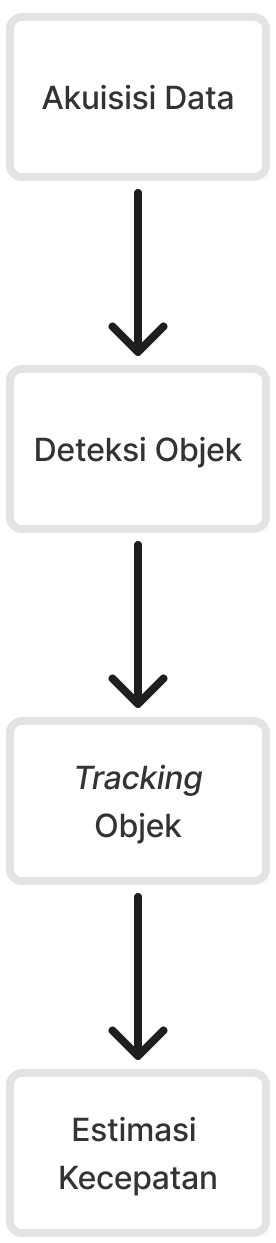
\includegraphics[width=0.1\textwidth]{gambar/diagramsistem.jpg}
    \caption{System workflow diagram.}
    \label{fig:system-arch}
\end{figure}

\subsection{Video Acquisition and Annotation}

Video is acquired using a DJI Phantom 4 Pro drone at various altitudes and lighting conditions. Annotation is conducted on Roboflow to prepare the dataset for training the YOLOv8 model.

\begin{figure}[H]
    \centering
    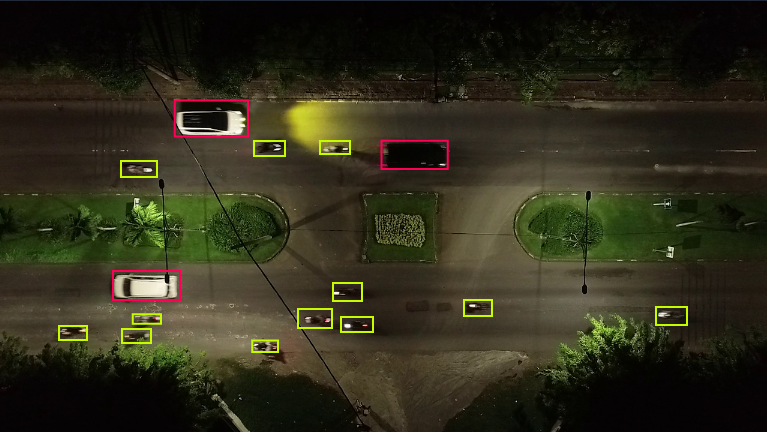
\includegraphics[width=0.45\textwidth]{gambar/anotasidatamalam.png}
    \caption{Example of annotated dataset (night).}
    \label{fig:annot-night}
\end{figure}

\begin{figure}[H]
    \centering
    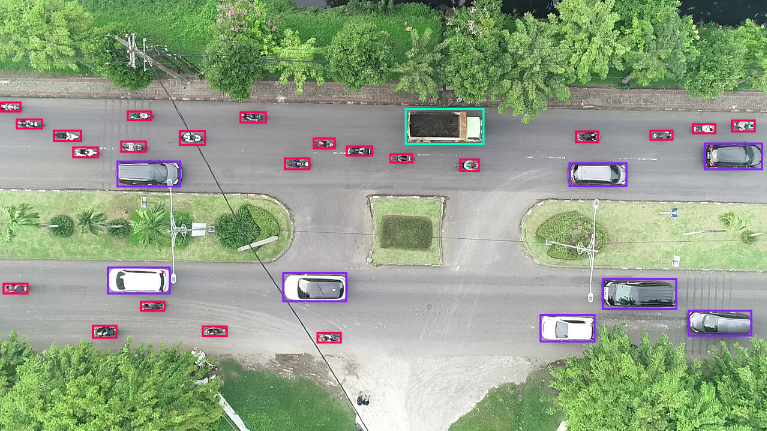
\includegraphics[width=0.45\textwidth]{gambar/anotasidatasiang.png}
    \caption{Example of annotated dataset (day).}
    \label{fig:annot-day}
\end{figure}

\subsection{Object Detection with YOLOv8-TensorRT}

Object detection is performed on video frames captured by a DJI Phantom 4 Pro drone, configured to record at a resolution of 720p and 30 FPS. The live video is transmitted to the Jetson Nano via RTMP streaming protocol, where real-time object detection is executed using a YOLOv8 model that has been converted into TensorRT format for efficient inference.

To reduce the processing load on the Jetson Nano, the video resolution is downscaled to 360p before inference. The YOLOv8 model has been trained to detect specific vehicle classes including cars, motorcycles, and trucks. Upon detection, each object is labeled and enclosed within a bounding box according to its classification.

The detection model only processes objects with a confidence threshold above 0.45, and bounding boxes are rendered for objects exceeding this threshold. Figure \ref{fig:deteksiobjek} shows an example of successful object detection on video frames using YOLOv8 in TensorRT format.

\begin{figure}[H]
    \centering
    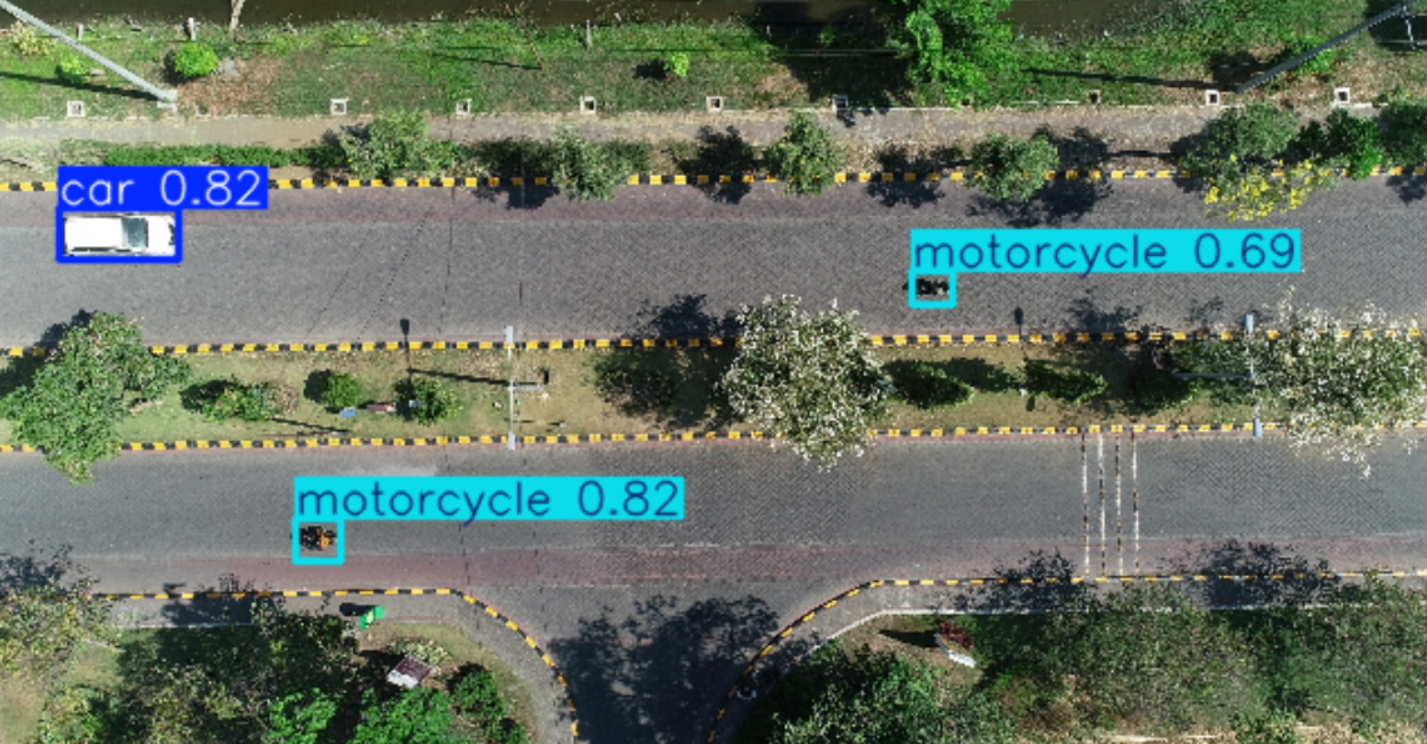
\includegraphics[width=0.45\textwidth]{gambar/deteksiobjek.png}
    \caption{Object detection output using YOLOv8 with TensorRT.}
    \label{fig:deteksiobjek}
\end{figure}


\subsection{Object Tracking with OC-SORT}

After vehicle objects are detected in each frame, tracking is employed to maintain object identity across successive frames. Two tracking algorithms were considered in this study: OC-SORT and ByteTrack.

Experimental results showed a notable difference between the two methods. ByteTrack offers faster processing speed, but at the cost of reduced tracking accuracy. In particular, ByteTrack occasionally fails to consistently assign bounding boxes to all detected objects, leading to incomplete tracking information.

Due to these limitations, this system utilizes the OC-SORT (Observation-Centric SORT) algorithm for object tracking. OC-SORT maintains better temporal consistency in assigning IDs to objects and performs well in aerial imagery scenarios where consistent motion patterns and occlusions are common.

To identify tracked objects uniquely, the center point of each bounding box is calculated using geometric midpoint formulas. This center is defined by:

\begin{equation}
    x_c = \frac{x_{min} + x_{max}}{2}, \quad
    y_c = \frac{y_{min} + y_{max}}{2}
\end{equation}

where $(x_{min}, y_{min})$ and $(x_{max}, y_{max})$ are the top-left and bottom-right coordinates of the bounding box. Each object is assigned a unique tracking ID along with its detected class label, allowing consistent tracking over time.

\subsection{Speed Estimation Process}

Once the objects are detected and tracked across frames, the system proceeds to estimate their speed. The movement of each object is calculated based on the displacement of its center point across frames using the Euclidean distance formula:

\begin{equation}
\label{eq:euclidean}
d = \sqrt{(x_2 - x_1)^2 + (y_2 - y_1)^2}
\end{equation}

where $(x_1, y_1)$ and $(x_2, y_2)$ represent the center coordinates of an object in two consecutive frames. This pixel-based displacement is then converted to meters using a scale factor derived from the Ground Sampling Distance (GSD) or Pixels per Meter (PPM), as shown in Table~\ref{tbl:skala_ppm}.

\begin{table}[H]
\centering
\caption{Meter-per-pixel scale based on drone altitude}
\label{tbl:skala_ppm}
\begin{tabular}{|c|c|}
\hline
\textbf{Altitude (m)} & \textbf{Meter per Pixel} \\ \hline
20 & 1 : 21.44 \\ \hline
30 & 1 : 14.30 \\ \hline
40 & 1 : 10.72 \\ \hline
\end{tabular}
\end{table}

To compute the object’s speed in kilometers per hour (km/h), the system applies the following equation:

\begin{equation}
\label{eq:speed_ms}
v = \frac{d}{t} \times 3.6
\end{equation}

where $d$ is the real-world displacement in meters (converted from pixels), $t$ is the time interval in seconds between frames, and $v$ is the estimated speed in km/h. The multiplier 3.6 converts speed from meters per second (m/s) to kilometers per hour (km/h), as commonly used in vehicle speedometers.

This method enables the system to estimate the vehicle's speed solely based on visual information from drone footage, making it suitable for flexible, infrastructure-free deployment.

\subsection{Streaming Setup}

The computation platform used in this study is the NVIDIA Jetson Nano, which acts as an edge device for running the detection, tracking, and speed estimation processes. The drone (DJI Phantom 4 Pro) transmits video streams via the Real-Time Messaging Protocol (RTMP). A shared network is established to ensure that the Jetson Nano is able to access the stream through a consistent IP configuration.

An RTMP server is configured using MediaMTX on a laptop. The drone sends its video feed to this server, and the Jetson Nano pulls the stream using FFmpeg integrated with OpenCV. The data transmission flow is illustrated in Figure~\ref{fig:alurdata}.

\begin{figure}[H]
    \centering
    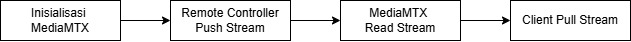
\includegraphics[width=0.45\textwidth]{gambar/pengirimandata.jpg}
    \caption{RTMP-based data transmission flow using MediaMTX.}
    \label{fig:alurdata}
\end{figure}

As shown in Figure~\ref{fig:alurdata}, the MediaMTX server is initialized on the laptop, and all devices are configured within the same local network. The Jetson Nano operates as the RTMP client, enabling it to receive and process the real-time video stream.

\subsection{System Processing Flow}

The core algorithm of the speed estimation program consists of several sequential stages, including frame acquisition, detection, tracking, and estimation. These components are implemented using a multithreaded pipeline for performance optimization. The processing flow of the system is illustrated in Figure~\ref{fig:diagramproses}.

\begin{figure}[H]
    \centering
    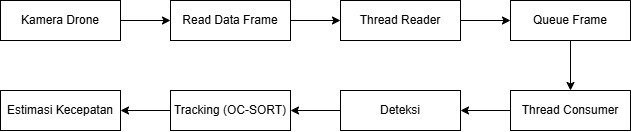
\includegraphics[width=0.45\textwidth]{gambar/algoritma.jpg}
    \caption{Program workflow for detection, tracking, and speed estimation.}
    \label{fig:diagramproses}
\end{figure}

\subsection{Hardware Topology}

The hardware configuration consists of the drone, a smartphone for controller interface, a laptop as the RTMP server, and the Jetson Nano as the inference device. The complete hardware topology is illustrated in Figure~\ref{fig:topologihardware}.

\begin{figure}[H]
    \centering
    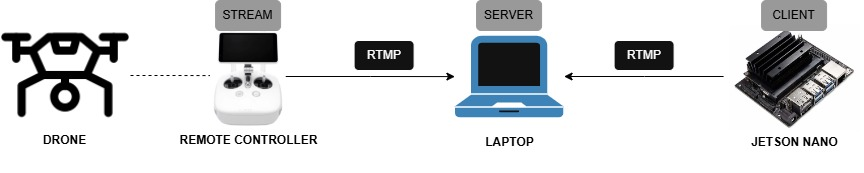
\includegraphics[width=0.45\textwidth]{gambar/topologi-hardware.jpg}
    \caption{Hardware topology for field deployment.}
    \label{fig:topologihardware}
\end{figure}

As shown in Figure~\ref{fig:topologihardware}, the RTMP protocol plays a central role in linking the drone's video feed to the Jetson Nano, enabling direct video input for on-site inference. This configuration allows for portable, real-time processing and visualization.

\subsection{Platform Specification}

The final system is deployed on a Jetson Nano using Ubuntu OS, CUDA, TensorRT, OpenCV, and PyTorch. RTMP stream is handled with FFmpeg and processed using OpenCV.

\begin{table}[H]
\centering
\caption{Jetson Nano Specification}
\label{tab:jetson-specs}
\begin{tabular}{|l|l|}
\hline
\textbf{Component} & \textbf{Specification} \\ \hline
CPU & Quad-core ARM Cortex-A57 @ 1.43 GHz \\ \hline
GPU & 128-core Maxwell NVIDIA GPU \\ \hline
Memory & 4 GB LPDDR4 RAM \\ \hline
Storage & microSD card slot (supports up to 64 GB) \\ \hline
\end{tabular}
\end{table}

